%-------------------- Document-wide settings --------------------%
\documentclass[aspectratio=1610,12pt,dvipsnames]{beamer}

\usepackage[font=small,skip=2pt]{caption}
\captionsetup[figure]{labelformat=empty}

\usetheme{Warsaw}

\setbeamertemplate{navigation symbols}{}
\setbeamertemplate{footline}
{
  \leavevmode%
  \hbox{%
  \begin{beamercolorbox}[wd=.4\paperwidth,ht=2.25ex,dp=1ex,center]{author in head/foot}%
    \usebeamerfont{author in head/foot}\insertshortauthor
  \end{beamercolorbox}%
  \begin{beamercolorbox}[wd=.6\paperwidth,ht=2.25ex,dp=1ex,center]{title in head/foot}%
    \usebeamerfont{title in head/foot}\insertshorttitle\hspace*{3em}
    \insertframenumber{} / \inserttotalframenumber\hspace*{1ex}
  \end{beamercolorbox}}%
  \vskip0pt%
}

\usepackage{listings,graphicx,verbatimbox,hyperref}
\usepackage{hyperref}
%\usepackage{bibentry}
% \usepackage[customcolors,shade]{hf-tikz}
% \usepackage{tikz}
\usepackage{amsmath}
\usepackage{xcolor}

\newcommand*{\colorboxed}{}
\def\colorboxed#1#{%
  \colorboxedAux{#1}%
}
\newcommand*{\colorboxedAux}[3]{%
  % #1: optional argument for color model
  % #2: color specification
  % #3: formula
  \begingroup
  \colorlet{cb@saved}{.}%
  \color#1{#2}%
  \boxed{%
    \color{cb@saved}%
    #3%
  }%
  \endgroup
}

\usepackage[style=nature]{biblatex}
\DeclareCiteCommand{\footcite}[\mkbibfootnote]
  {\usebibmacro{prenote}}
  {\printnames[family-given]{labelname}%
   \hspace{1mm} \printfield{journaltitle}%
   \hspace{1mm} \printfield{year}}
  {\addsemicolon\space}
  {\usebibmacro{postnote}}


\newcommand{\N}{\mathbb{N}}
\newcommand{\Z}{\mathbb{Z}}
\newcommand{\Q}{\mathbb{Q}}
\newcommand{\R}{\mathbb{R}}
\newcommand{\C}{\mathbb{C}}
\newcommand{\norm}[1]{\left\lVert#1\right\rVert}
\newcommand{\ceil}[1]{\lceil#1\rceil}
\newcommand{\ov}{\overline}
\newcommand{\cleq}{\preccurlyeq}
\newcommand{\cgeq}{\succcurlyeq}
\newcommand{\bdy}{\textbf{\text{Bdy}}}
\newcommand{\trace}{\text{trace}}
\newcommand{\dom}{\textbf{dom}}
\newcommand{\expec}{\mathbb{E}}
\newcommand{\bigO}{\mathcal{O}}
\newcommand{\tr}{\text{tr}}
\newcommand{\<}{\langle}
\renewcommand{\>}{\rangle}
\newcommand*\oldmacro{}%
\let\oldmacro\insertshorttitle%
\DeclareMathOperator*{\argmax}{arg\,max}
\DeclareMathOperator*{\argmin}{arg\,min}


\date{\today}

\addbibresource{NOGA-UA-gas/bib/gas.bib}
\addbibresource{LearningTetradPaper/refs.bib}

\begin{document}
%------------------------------------------------------------------%

%-------------------- Presentation big picture --------------------%
\title{Comprehensive Exam}
\author{Criston Hyett}
\graphicspath{{./figs/}}
%------------------------------------------------------------------%
\begin{frame}
  \maketitle
\end{frame}
% ------------------------------------------------------------------%

% ------------------------------------------------------------------%
\begin{frame}{Overview}
  \begin{figure}
    \centering
    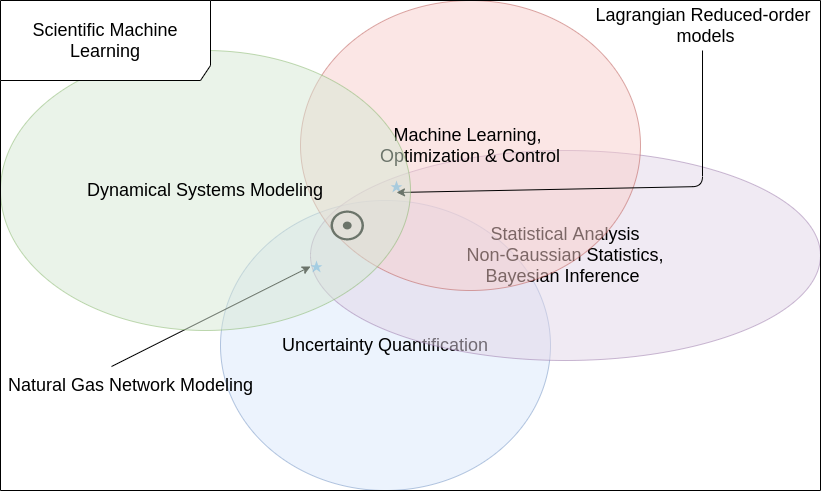
\includegraphics[width=0.8\textwidth]{overview.png}
  \end{figure}
\end{frame}
% ------------------------------------------------------------------%

%-------------------- NOGA UA Gas Modeling ------------------------%

\title[Control of Line Pack in Natural Gas System of Israel]{Control of Line Pack in Natural Gas System of Israel:
Balancing Limited Resources under Uncertainty}
\author[Hyett, Pagnier, Alisse, Saban, Goldshtein, Chertkov]{Criston Hyett, Laurent Pagnier, Jean Alisse, Lilah Saban, Igal Goldshtein, Misha Chertkov}

\institute{The University of Arizona \& NOGA Israel}

\graphicspath{{./NOGA-UA-gas/figs/}}
% -------------------------------------------------------------------------------%
\begin{frame}
  \maketitle
\end{frame}
% -------------------------------------------------------------------------------%
% -------------------------------------------------------------------------------%
\begin{frame}{Context}
  \begin{columns}
    \begin{column}{0.5\textwidth}
      \begin{figure}
        \centering
        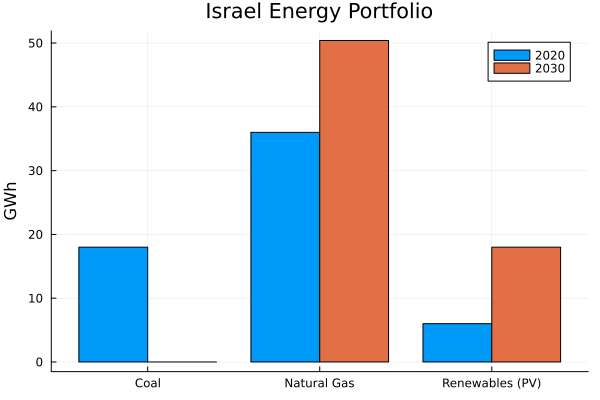
\includegraphics[width=\textwidth]{energyPortfolio.png}
      \end{figure}
    \end{column}

    \begin{column}{0.5\textwidth}
      \begin{figure}
        \centering
        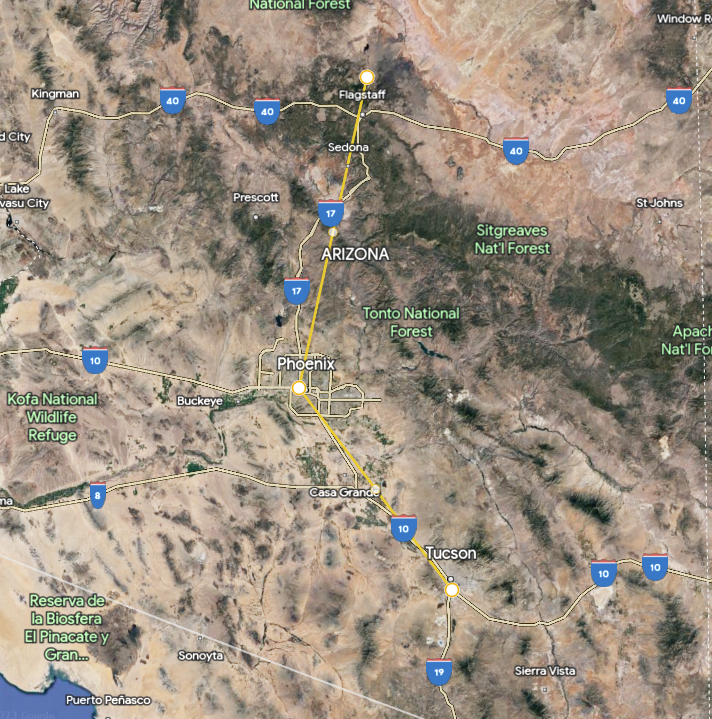
\includegraphics[width=0.75\textwidth]{israelLengthOnAZ.png}
      \end{figure}
    \end{column}
  \end{columns}
\end{frame}
% -------------------------------------------------------------------------------%

% -------------------------------------------------------------------------------%
\begin{frame}{Project Goals}
  \begin{itemize}
  \item Operations-aware modeling and simulation of a reduced model of Israel's natural gas network.
    \begin{itemize}
    \item Flux control at inlet nodes
    \item Realistic initial conditions
    \item Assessing relevant challenges
      \begin{itemize}
      \item Robustness in the case of uncertain PV generation
      \item Robustness in the case of an insult to the system
      \end{itemize}
    \end{itemize}

  \item Model \& open-source tool development
    \begin{itemize}
    \item Solver suite specifically suited to the needs of natural gas networks
    \item Advanced automatic controls
    \item Monte-Carlo/Uncertainty Quantification
    \end{itemize}
  \end{itemize}
\end{frame}
% -------------------------------------------------------------------------------%

% -------------------------------------------------------------------------------%
\begin{frame}{Reduced Model of Israel's Gas Network}
  \begin{center}
    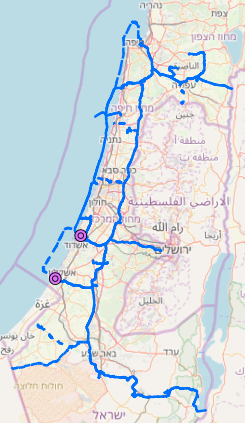
\includegraphics[width=0.25\textwidth]{fullModel.png}
    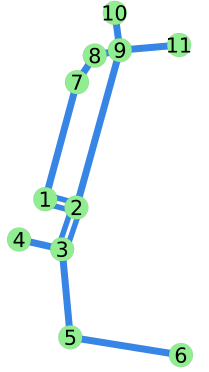
\includegraphics[width=0.25\textwidth]{reducedModel.png}
  \end{center}
  \footnotetext{\url{https://www.gov.il/he/departments/guides/distribution_area}}
\end{frame}
% -------------------------------------------------------------------------------%

% -------------------------------------------------------------------------------%
\begin{frame}{Effective Gas Flow Equations}
  Under reasonable assumptions, the system of PDEs governing gas flow is 
  \begin{align}
    \partial_t \rho & + \partial_x \phi = 0\\
    \partial_t \phi & + \partial_x P = -\beta \frac{\phi|\phi|}{\rho}
  \end{align}
  These, supplemented with initial
  \begin{align}
    \rho(x,0) &= \rho_0(x)\\
    \phi(x,0) &= \phi_0(x)
  \end{align}
  and boundary conditions at each node
  \begin{equation}
    \rho_i(t) \text{ \emph{or} } \phi_i(t)
  \end{equation}
  and an equation of state relating pressure and density
  \begin{equation}
    P(\rho) = ... \quad \rho(P) = ...
  \end{equation}
\end{frame}
% -------------------------------------------------------------------------------%

% -------------------------------------------------------------------------------%
\begin{frame}{Staggered Grid Method}
  \begin{columns}
    \begin{column}{0.6\textwidth}
      \begin{figure}
        \centering
        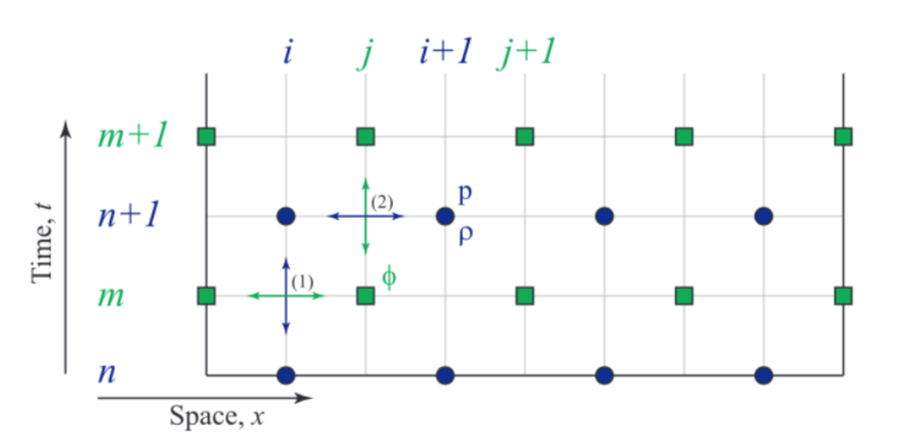
\includegraphics[width=1.0\textwidth]{ScenarioResults/staggeredGrid.png}
        \caption{Figure taken from Gyrya,Zlotnik: "An explicit staggered-grid method for numerical simulation of large-scale natural gas pipeline networks"}
        \label{fig:my_label}
      \end{figure}
    \end{column}

    \begin{column}{0.4\textwidth}
      \begin{equation*}
        \color{blue} \partial_t \rho + \partial_x \phi = 0
      \end{equation*}
      \begin{equation*}
        \color{ForestGreen} \partial_t \phi + \partial_x P = -\beta \frac{\phi|\phi|}{\rho}
      \end{equation*}
      CFL stability condition:
      \begin{equation*}
        \sqrt{P'(\rho)} \frac{\Delta t}{\Delta x} \leq 1
      \end{equation*}
    \end{column}
  \end{columns}
\end{frame}
% -------------------------------------------------------------------------------%

% -------------------------------------------------------------------------------%
\begin{frame}{Results: Scenario 1}
  \begin{figure}
    \centering
    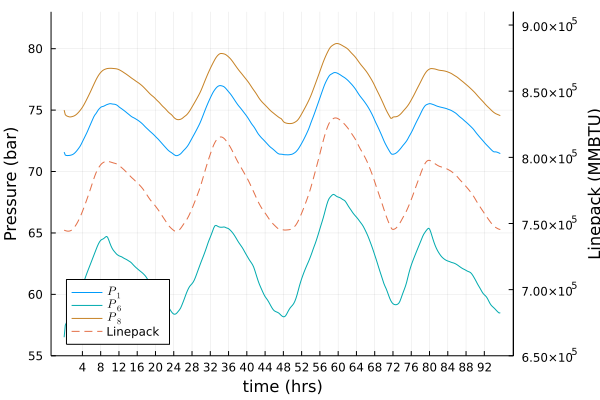
\includegraphics[width=0.65\textwidth]{ScenarioResults/scen1.png}
    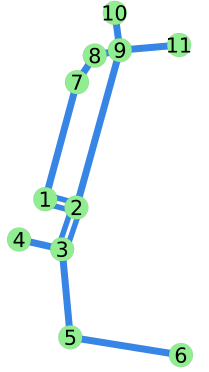
\includegraphics[width=0.25\textwidth]{reducedModel.png}
    \caption{Nominal week in August.}
  \end{figure}
\end{frame}
% -------------------------------------------------------------------------------%

% -------------------------------------------------------------------------------%
\begin{frame}{Uncertainty}
  Moderate uncertainty at demand nodes is represented through addition of a random noise at the consumption site
  \begin{equation}
    d_i(t) \to X_i(t)
  \end{equation}
  where
  \begin{equation}
    dX_i(t) = \alpha(d_i(t) - X_i(t))dt + \gamma dW
  \end{equation}
  is a Ornstein–Uhlenbeck process
  \begin{itemize}
  \item $\mathbb{E}[X_i(t)] = d_i(t)$
    \vspace{0.1cm}
  \item $ \text{Var}(X_i(t)) = \frac{\gamma}{2\alpha}\left(1 - e^{-2\alpha t} \right) $
    \vspace{0.1cm}
  \item The parameters were tuned heuristically to ensure the mean was respected, and the variance approaches
    \begin{equation}
      \text{Var}(X_i(t)) \approx 0.01 \mu_i^2
    \end{equation}
    With $\mu_i$ being the mean withdrawal of node $i$.
  \end{itemize}

\end{frame}
% -------------------------------------------------------------------------------%


% -------------------------------------------------------------------------------%
\begin{frame}{Results: Scenario 2}
  \begin{figure}
    \centering
    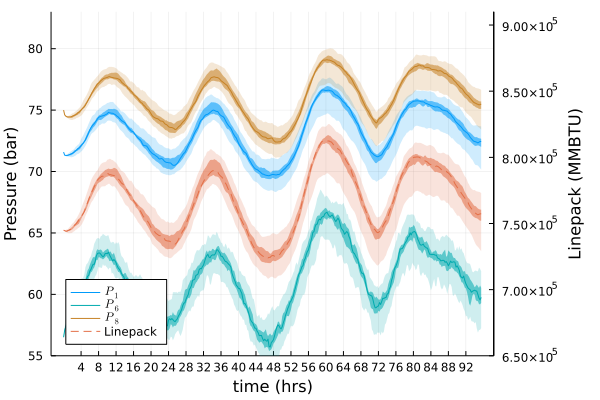
\includegraphics[width=0.65\textwidth]{ScenarioResults/scen2.png}
    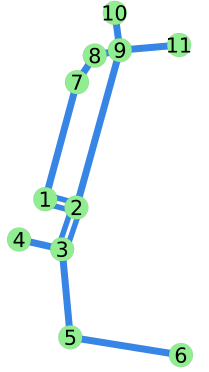
\includegraphics[width=0.25\textwidth]{reducedModel.png}
    \caption{Linepack and pressures for random perturbation on top of nominal August days.}
  \end{figure}
\end{frame}
% -------------------------------------------------------------------------------%

% -------------------------------------------------------------------------------%
\begin{frame}{Results: Scenario 3 \& 4}
  \begin{figure}
    \centering
    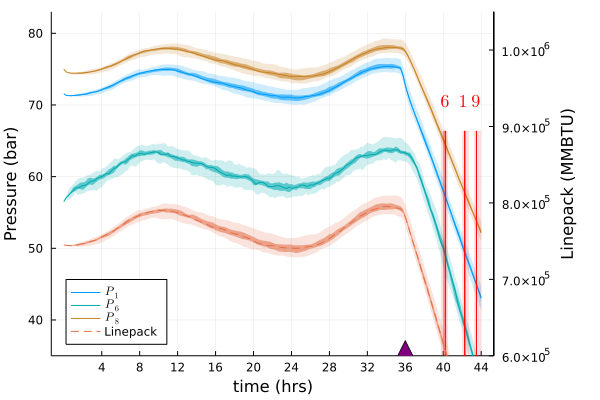
\includegraphics[width=0.45\textwidth]{ScenarioResults/scen3.png}\hspace{0.6cm}%
    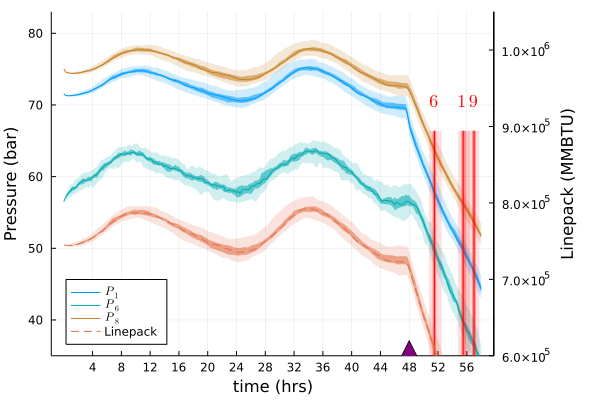
\includegraphics[width=0.45\textwidth]{ScenarioResults/scen4.png}
    \caption{Linepack and pressures responding to loss of supply at node 1. (Left) shows the insult at a peak of intraday linepack, and (right) shows the same insult at the trough.}
  \end{figure}
  \begin{columns}
    \begin{column}{0.5\textwidth}
      \begin{equation*}
        \tau = 4.13 \pm 0.38 \text{ hrs}
      \end{equation*}
    \end{column}

    \begin{column}{0.5\textwidth}
      \begin{equation*}
        \tau = 3.58 \pm 0.89 \text{ hrs}
      \end{equation*}
    \end{column}
  \end{columns}
\end{frame}
% -------------------------------------------------------------------------------%


% -------------------------------------------------------------------------------%
\begin{frame}{Results: Scenario 5}
  \begin{figure}
    \centering
    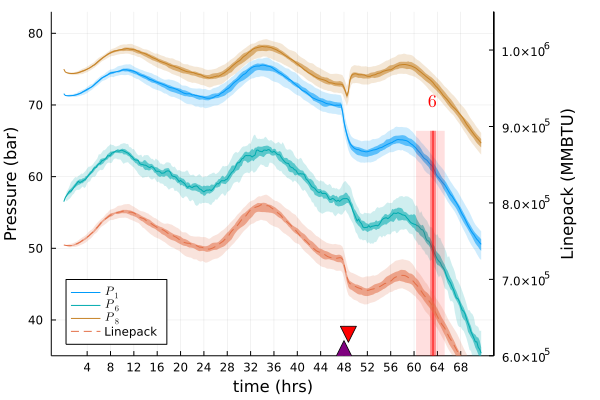
\includegraphics[width=0.65\textwidth]{ScenarioResults/scen5.png}
    \caption{Linepack and pressures for insult at hour 48, implementing a max-flow control on the remaining supply at node 8. $\tau = 14.17 \pm 4.07 \text{ hrs}$}
  \end{figure}
\end{frame}
% -------------------------------------------------------------------------------%

% -------------------------------------------------------------------------------%
\begin{frame}{Results: Scenario 6}
  \begin{figure}
    \centering
    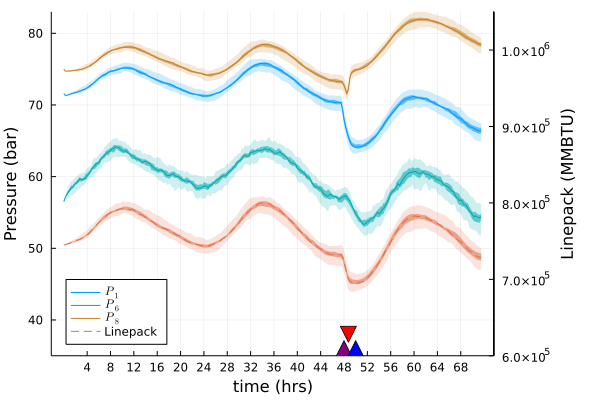
\includegraphics[width=0.65\textwidth]{ScenarioResults/scen6.png}
    \caption{Linepack and pressures for insult at hour 48, implementing a max-flow control on the remaining supply at node 8, and curtailing demand 2 hours after the insult.}
  \end{figure}
\end{frame}
% -------------------------------------------------------------------------------%

%-------------------------------------------------------------------------------%
\begin{frame}{Next Steps}
  \begin{itemize}
  \item Better UQ: Stochastic Finite Volumes(?)
  \item Higher order method and efficient implementation to allow for parallelization and acceleration.
  \item Advanced automatic controls
    \begin{itemize}
    \item This would mimick some actual protocol, and allow you to make statements such as, "with 95\% confidence, using protocol A, the natural gas system is robust to an insult of type B"
    \end{itemize}
  \item Simulation and optimization of the joint power and gas grids, under uncertainty.
  \end{itemize}
\end{frame}
%-------------------------------------------------------------------------------%

%-------------------------------------------------------------------------------%
\begin{frame}{Questions/Comments/Suggestions?}
  \begin{itemize}
  \item cmhyett@math.arizona.edu
  \item \url{https://arxiv.org/abs/2304.01955}
  \item \url{https://github.com/cmhyett/FluxControlLinepack}
  \end{itemize}  
\end{frame}
% -------------------------------------------------------------------------------%

%-------------------- Turbulence ----------------------------------%
The dynamics of the velocity gradient tensor provide a privileged view into important characteristics of turbulence, some of which include: local fluid deformation, strain, energy cascade, and intermittency. Recent work using Tensor Basis Neural Network for the evolution of the velocity gradient tensor has performed very well. In this work we closely examine the individual contributions from the components of this physics-informed machine learning framework in search of interpretability. We find that not all components contribute to the prediction, and thus an even simpler description is possible. We conclude by postulating physical justification of this further-reduced description.

\subsection{Introduction}
Turbulence being a widespread phenomenon, an enormous body of work is dedicated to modeling and simulating it. Resulting from this plethora of simulation efforts are enormous datasets. Recently, with the advances of machine learning - particularly physics-informed machine learning - data-driven models regularly out-perform phenomenological models, suggesting that these large datasets contain exploitable patterns that we don't yet recognize.

At the same time, the promise of physics-informed machine learning is that via imposing structure on the infuriatingly flexible neural network, one might simultaneously improve generalizability (i.e., learn not just data patterns, but physical laws), and have those learned models be interpretable.

Our work focuses on the Lagrangian perspective of turbulence, centering ourselves on the statistical evolution of the velocity gradient tensor (VGT). Recent work \cite{tian2021} constructed the so called ``Tensor Basis Neural Network'' (TBNN), and trained it to learn the pressure Hessian contribution to the evolution of the VGT.

In this work we will present the TBNN formulation, reiterate the results of Tian et.al, and show that by examining the trained model, one can tease out physically relevant patterns, toward the hope of learning new physics.


\subsection{Tensor Basis Neural Network}
We begin with Navier-Stokes for an incompressible fluid:
\begin{equation} \label{eq:NS}
  \frac{\partial u_i}{\partial t} + u_k \frac{\partial u_i}{\partial x_k} = -\frac{\partial P}{\partial x_i} + \nu \frac{\partial^2 u_i}{\partial x_k \partial x_k}
\end{equation}
then, as the velocity gradient tensor is defined as $A_{ij} = \frac{\partial u_i}{\partial x_j}$, we apply spatial derivatives, and use the definition of material derivative ($\frac{dA_{ij}}{dt} = \frac{\partial A_{ij}}{\partial t} + u_k\frac{\partial A_{ij}}{\partial x_k}$) to get:
\begin{equation}
  \frac{dA_{ij}}{dt} = \frac{\partial A_{ij}}{\partial t} + u_k \frac{\partial A_{ij}}{\partial x_k} = - A_{ik}A_{kj} - \frac{\partial^2 P}{\partial x_i \partial x_j} + \nu \frac{\partial^2 A_{ij}}{\partial x_k \partial x_k}
\end{equation}
Additionally, from incompressibility, we have
\begin{equation}
  \frac{\partial^2 P}{\partial x_k \partial x_k} = - A_{ij}A_{ji}
\end{equation}
This allows us to define the nonlocal deviatoric part of the pressure hessian
\begin{equation}
  H_{ij} = - \left( \frac{\partial^2 P}{\partial x_i \partial x_j} - \frac{1}{3}\frac{\partial P}{\partial x_k \partial x_k}\delta_{ij}  \right)
\end{equation}

We can write the formal (nonlocal) solution for the deviatoric pressure hessian as\cite{ohkitani1995}

\begin{equation}
  H_{ij}(\textbf{x}) = \iiint \frac{\delta_{ij} - \hat{r_i}\hat{r_j}}{2\pi r^3}Q(\textbf{x} + \textbf{r})d\textbf{r}
\end{equation}

Following Lawson \& Dawson\cite{lawson2015}, an expansion of the integral is proposed, first as a Taylor series expansion in $Q(x+r)$
\begin{equation}
  \hat{H} = \sum_{m,n = 0}^\infty \alpha_{mn}S^mW^n
\end{equation}
where
\begin{equation}
  S = \frac{1}{2}(A + A^T) \qquad W = \frac{1}{2}(A - A^T)
\end{equation}

Finally we can reduce from an infinite sum using Cayley-Hamilton, and expand via the tensor basis\cite{zheng1993}
\begin{equation}
  \hat{H} = \sum_{n=1}^{10} g^{(n)}(\lambda_1, \dots, \lambda_5)T^{(n)}
\end{equation}
with $g^{(n)}$ scalar functions of the invariants
\begin{small}
  \begin{equation*}
    \lambda_1 = \tr(S^2) \quad \lambda_2 = \tr(W^2) \quad \lambda_3 = \tr(S^3) \quad \lambda_4 = \tr(W^2S) \quad \lambda_5 = \tr(W^2S^2)
  \end{equation*}
\end{small}
and the tensor basis given by:
\begin{small}
  \begin{align*}
    &T^{(1)} = S &T^{(2)} &= SW-WS\\
    &T^{(3)} = S^2 - \frac{1}{3}I \cdot \tr(S^2) &T^{(4)} &= W^2 - \frac{1}{3}I \cdot \tr(W^2)\\
    &T^{(5)} = WS^2 - S^2W &T^{(6)} &= W^2S + SW^2 - \frac{2}{3}I \cdot \tr(SW^2)\\
    &T^{(7)} = WSW^2-W^2SW &T^{(8)} &= SWS^2 - S^2WS\\
    &T^{(9)} = W^2S^2 + S^2W^2 - \frac{2}{3}I \cdot \tr(S^2W^2) &T^{(10)} &= WS^2W^2 - W^2S^2W
  \end{align*}
\end{small}
We use the natural timescale $\tau = \langle \norm{S^2}_2 \rangle^{-1}$ to normalize our VGT, and thus all of the $\lambda_i, T^{(j)}$.
This formulation reduces the challenge to finding the functions of known scalars, i.e., learning the $g^{(n)}$'s.

\begin{equation}
  \hat{H} = \sum_{i=1}^{10} g_{\theta}^{(i)}(\lambda_1, \dots, \lambda_5)\cdot \hat{T}^{(i)}(\hat{A})
\end{equation}

\begin{small}
  \begin{equation*}
    \lambda_1 = \tr(\hat{S}^2) \quad \lambda_2 = \tr(\hat{W}^2) \quad \lambda_3 = \tr(\hat{S}^3) \quad \lambda_4 = \tr(\hat{W}^2\hat{S}) \quad \lambda_5 = \tr(\hat{W}^2\hat{S}^2)
  \end{equation*}
\end{small}
\begin{figure}
  \centering
  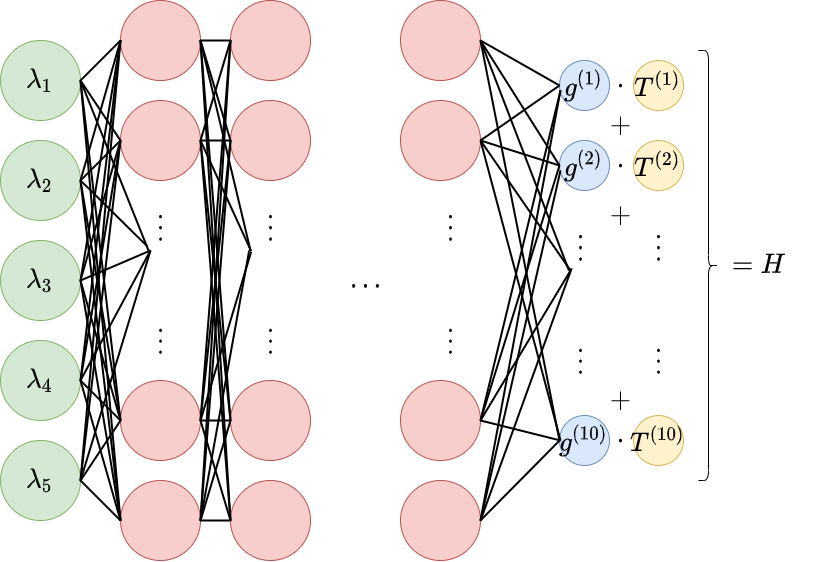
\includegraphics[width=0.5\textwidth]{./tbnn.png}
  \caption{Structure of TBNN}
  \label{fig:tbnn}
\end{figure}

\begin{equation}
  L(\theta) = \frac{1}{N}\sum^N\norm{\hat{H}_{\text{truth}} - \sum_{i=1}^{10}g_\theta^{(i)}(\lambda_1, \dots, \lambda_5)T^{(i)}}_2^2
\end{equation}




\subsection{Results}
Previous phenomenological models have used truncated tensor basis expansions, with constant coefficients fit from averaging over data, to model the pressure Hessian contribution. From investigating the trained parameterization of the full expansion, we can investigate these choices.

\begin{figure}
  \centering
  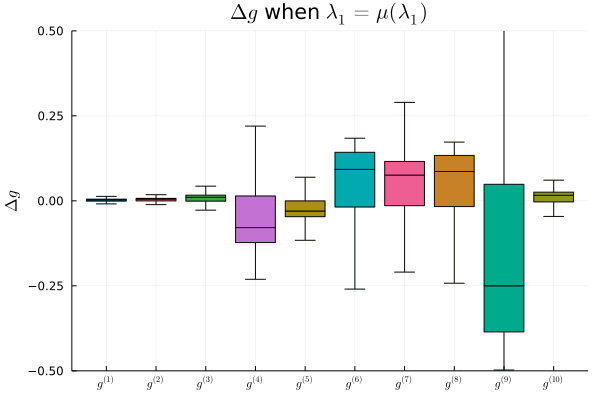
\includegraphics[width=0.5\textwidth]{./pi512/dgdl_1.png}%
  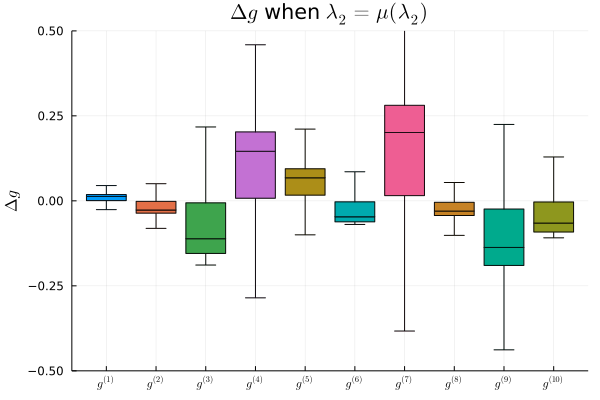
\includegraphics[width=0.5\textwidth]{./pi512/dgdl_2.png}
  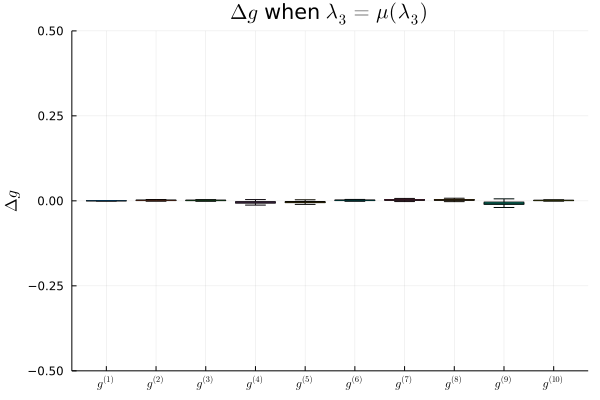
\includegraphics[width=0.5\textwidth]{./pi512/dgdl_3.png}%
  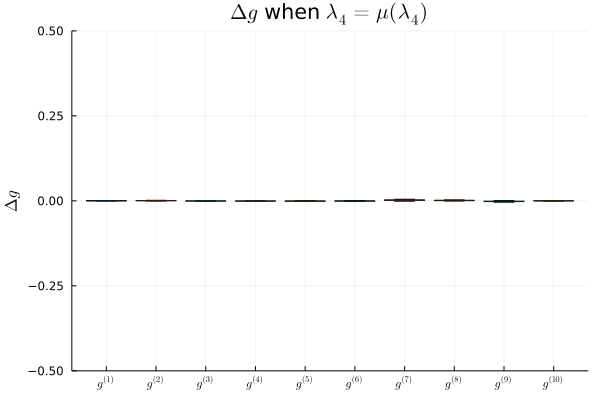
\includegraphics[width=0.5\textwidth]{./pi512/dgdl_4.png}
  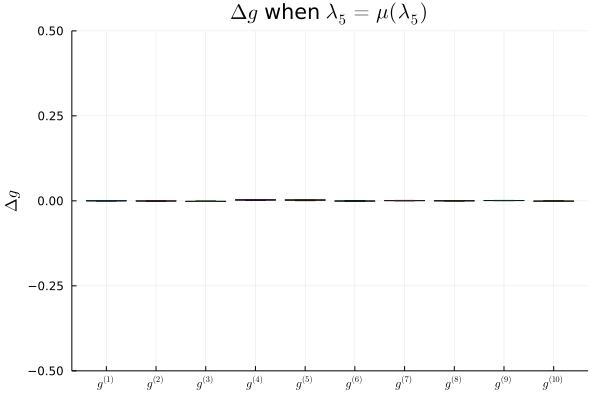
\includegraphics[width=0.5\textwidth]{./pi512/dgdl_5.png}
  \caption{ }
  \label{fig:sensitivityGs}
\end{figure}

To examine the learned model, we first investigate the sensitivity of the scalar functions $g_\theta^{(i)}$ to the variability of the invariants $\lambda_j$. This sensitivity will inform the learned ``importance'' of the $\lambda_i$ to each $g_\theta^{(i)}$. In particular, we see in figure \ref{fig:sensitivityGs} that $g^{(9)}$ has large sensitivity to changes in $\lambda_1$, while nearly no sensitivity to $\lambda_4$ or $\lambda_5$. In fact, all of the scalar functions seem to depend only on $\lambda_1, \lambda_2$. We can test this hypothesis by training a new TBNN using only the first two invariants. A comparison between the two predictions of the pressure Hessian contribution is shown in figure[\ref{fig:qrCMTComp}].

\begin{figure}
  \centering
  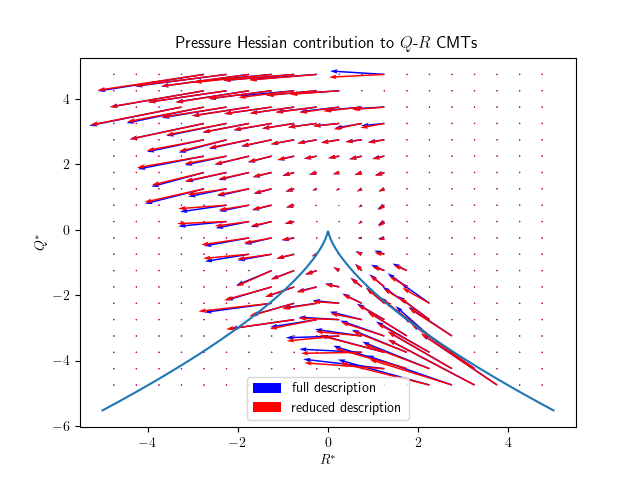
\includegraphics[width=0.75\textwidth]{./comp_qrCMT.png}
  \caption{ }
  \label{fig:qrCMTComp}
\end{figure}

We see that the change in prediction is very small - and within retraining error. Further, we can plot the $g$'s to investigate the functional dependence on the $\lambda_1,\lambda_2$, using k-nearest neighbors algorithm to interpolate between datapoints.

\begin{figure}
  \centering
  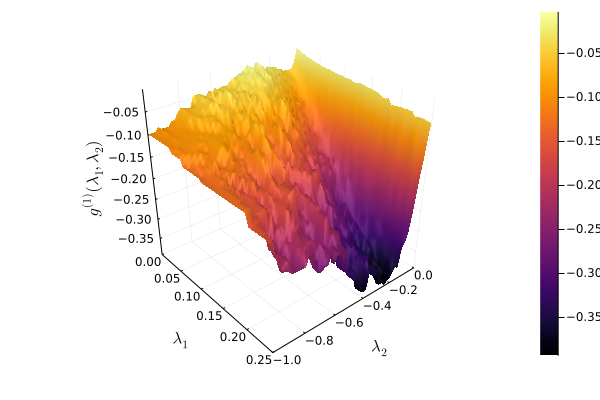
\includegraphics[width=0.33\textwidth]{./pi512/gFunctions/g1.png}%
  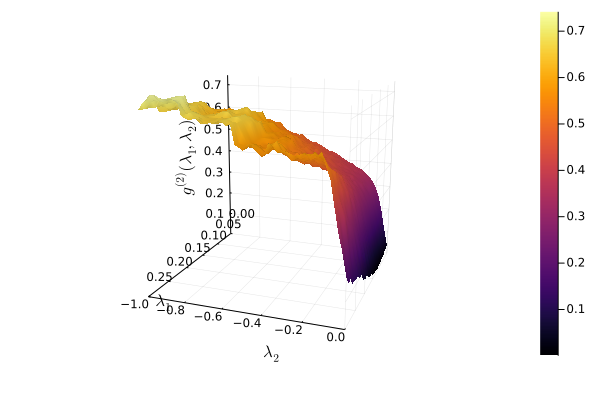
\includegraphics[width=0.33\textwidth]{./pi512/gFunctions/g2.png}%
  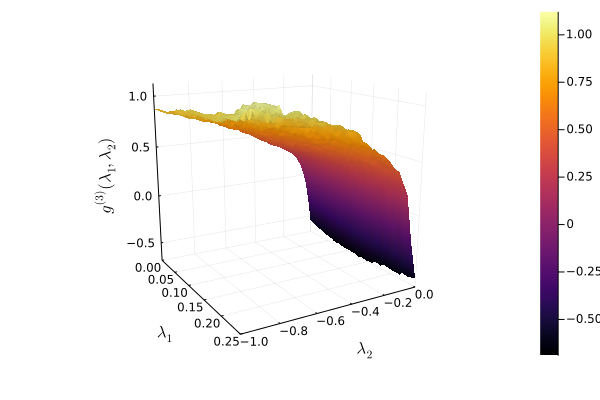
\includegraphics[width=0.33\textwidth]{./pi512/gFunctions/g3.png}
  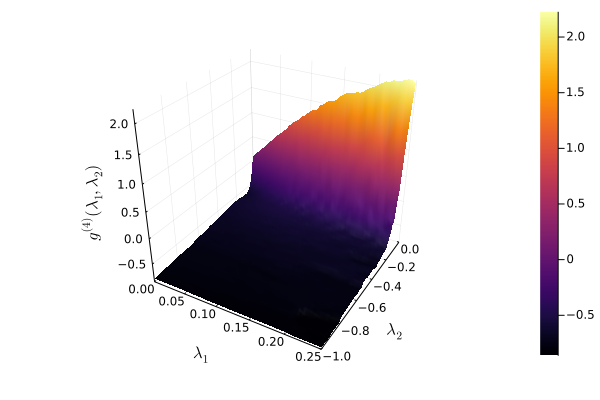
\includegraphics[width=0.33\textwidth]{./pi512/gFunctions/g4.png}%
  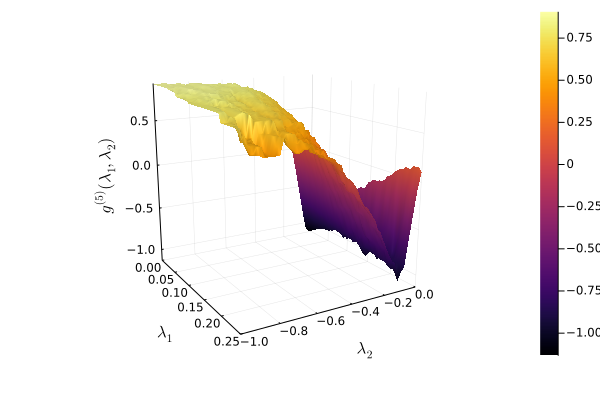
\includegraphics[width=0.33\textwidth]{./pi512/gFunctions/g5.png}%
  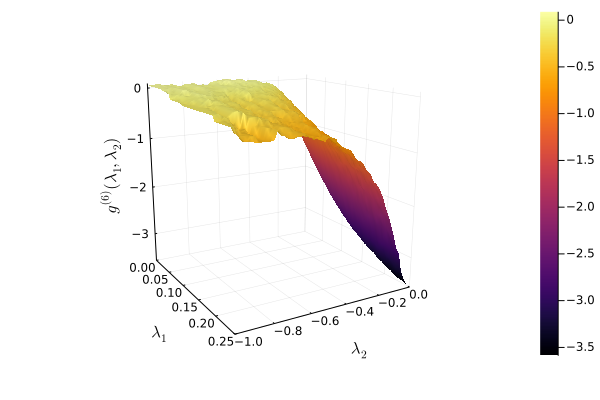
\includegraphics[width=0.33\textwidth]{./pi512/gFunctions/g6.png}
  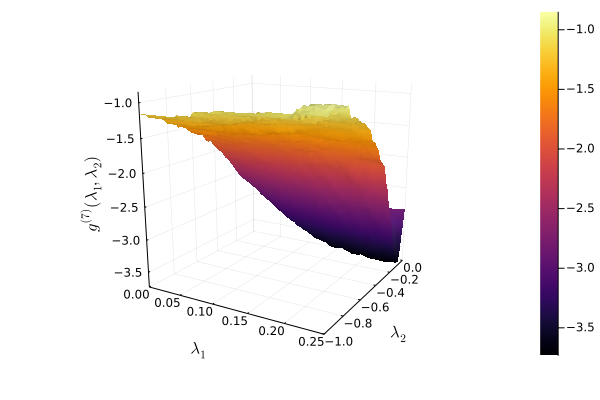
\includegraphics[width=0.33\textwidth]{./pi512/gFunctions/g7.png}%
  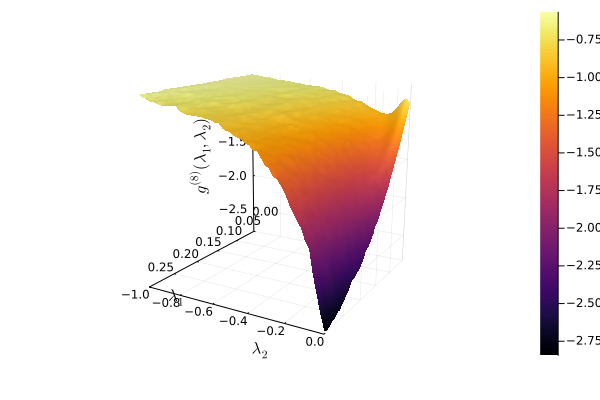
\includegraphics[width=0.33\textwidth]{./pi512/gFunctions/g8.png}%
  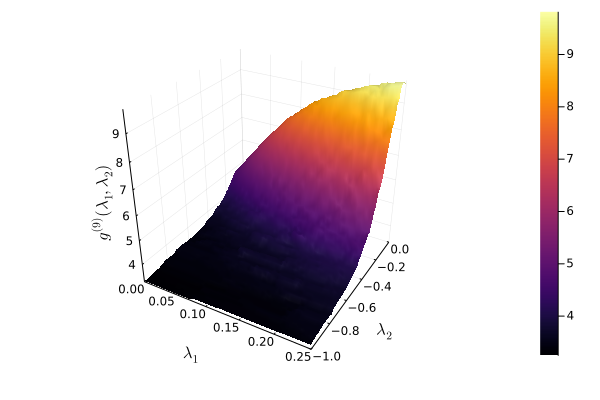
\includegraphics[width=0.33\textwidth]{./pi512/gFunctions/g9.png}
  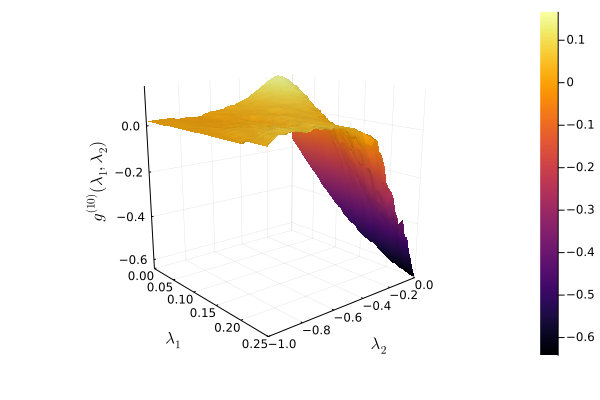
\includegraphics[width=0.33\textwidth]{./pi512/gFunctions/g10.png}%
  \caption{ }
  \label{fig:gFunctions}
\end{figure}


\subsection{Conclusion}
We investigate the spatiotemporal response of a reduced model of Israel's NG network to prescribed insults and human-in-the-loop controls in order to evaluate robustness and suggest control strategies. To reiterate, Israel's network is unique because of the absence of a compressor, and that the inlets specify flux, not pressure. Further, we perform this study looking towards the increased importance of NG to mitigate increasing stochasticity in demands expected in the coming years as coal is phased out, and renewables grow.

The specification of flux vs pressure leads to the pressure timeseries of the network being dominated by daily demand curves as shown in Fig.~(\ref{fig:scen1}), increasingly susceptible to pressure drift from stochastic fluctuations in nominal demands.

Further, we call out the importance of robustness of the network not simply to insults, but to insults at any time - leading to the idea of "system reserve" being time and spatially dependent.

Future work will improve on modeling to more completely capture uncertainty propagation through the network, and its influence and interaction with control strategies. We envision extending the prescribed control, also reinforced by monotonicity \cite{Vuffray2015Monotonicity,zlotnik_monotonicity_2016}, developed in this manuscript with the powerful optimization approaches developed to account for dynamic optimization over compressors \cite{rachford_optimizing_2000,carter_optimizing_2003,rachford_using_2009,zlotnik_optimal_2015,zlotnik_using_2016}, e.g. to evaluate benefits of adding compressors to the NG system of Israel. We also plan to carry on a comprehensive modeling and control of the combined power and gas system of Israel, in the spirit of the approach highlighted in \cite{carter_impact_2016,Zlotnik2017Coordinated}. 


%-------------------- References ----------------------------------%
\begin{frame}[allowframebreaks]{References}
  \nocite{tian2021}
  \nocite{chertkov1999}
  \printbibliography
   
    % \bibliographystyle{plain}
    % \bibliography{NOGA-UA-gas/bib/gas}
    % \end{tiny}
\end{frame}
% -----------------------------------------------------------------%

\end{document}